\subsection{Happy Waves: Unraveling Impedance with a Shorted 1/4-Wavelength Line!}

\begin{tcolorbox}[colback=gray!10, colframe=black, title=E9F09]  
What impedance does a 1/4-wavelength transmission line present to an RF generator when the line is shorted at the far end?

\begin{enumerate}[label=\Alph*.]
    \item \textbf{Very high impedance}
    \item Very low impedance
    \item The same as the characteristic impedance of the transmission line
    \item The same as the generator output impedance
\end{enumerate} \end{tcolorbox}

\subsubsection{Related Concepts}

To answer this question, it is essential to understand the behavior of transmission lines, particularly the concept of quarter-wavelength (1/4-wavelength) lines and their impedance properties.

A transmission line is characterized by its \textbf{characteristic impedance:} (\(Z_0\)), which is the impedance that the line presents to a signal propagating through it. When a transmission line is terminated with a load, the impedance seen looking into the transmission line can vary depending on the length of the line and the termination condition.

\subsubsection*{Impedance of a Shorted 1/4-Wavelength Transmission Line:}

For a 1/4-wavelength line (\(\lambda/4\)), the relationship between the load impedance (\(Z_L\)) and the input impedance (\(Z_{in}\)) looking towards the generator is given by the following formula:

\[
Z_{in} = \frac{Z_0^2}{Z_L}
\]

In this case, when the line is shorted at the far end, the load impedance \(Z_L\) is 0 (i.e., a short circuit). Therefore, substituting into the formula:

\[
Z_{in} = \frac{Z_0^2}{0}
\]

This expression indicates that the input impedance approaches infinity, or in practical terms, this means the line presents a very high impedance to the generator.

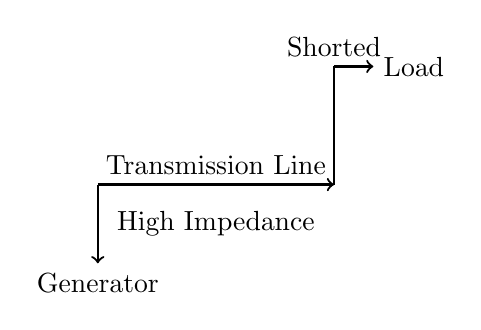
\begin{tikzpicture}
    \draw[->, thick] (0,0) -- (3,0) node[midway, above] {Transmission Line};
    \draw[thick] (3,0) -- (3,1.5) node[above] {Shorted};
    \draw[->, thick] (3,1.5) -- (3.5,1.5) node[right] {Load};
    \draw[->, thick] (0,0) -- (0,-1) node[below] {Generator};
    \node at (1.5, -0.5) {High Impedance};
\end{tikzpicture}

\subsubsection*{Conclusion:}

The answer to the question posed is \textbf{A: Very high impedance}. A clear understanding of transmission line theory and the specific behavior of a 1/4-wavelength line is crucial in RF communications. Recognition of the relationship between load impedance and input impedance is key to resolving many practical scenarios involving RF systems and their components.
